\documentclass{standalone}
\usepackage{tikz}
\usetikzlibrary{calc,patterns}
\begin{document}
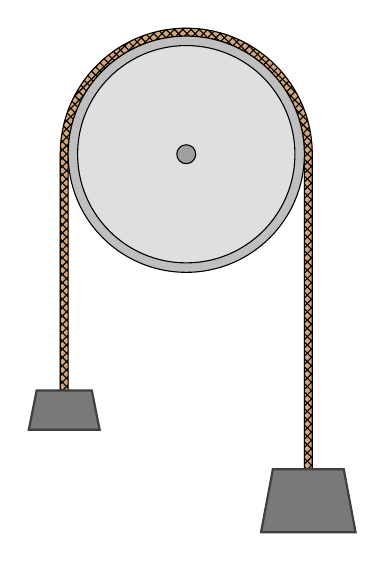
\begin{tikzpicture}
	\def\slength{3}
	\def\tlength{4}
	\def\pulleyradius{1.5}
	\def\ropethickness{.1}
	
	\coordinate (Pulley) at (0,0);
	\coordinate (Small) at (-\pulleyradius,-\slength);
	\coordinate (Big) at (\pulleyradius,-\tlength);

	\draw[fill, brown!70!white] (Small) -- ++(-\ropethickness,0) -- ++(0,\slength) arc[start angle = 180, end angle = 0, radius = {\pulleyradius + \ropethickness}] -- ++ (0,-\tlength) -- ++(-\ropethickness,0) -- ++ (0,\tlength) arc[start angle = 0, end angle = 180, radius = \pulleyradius] -- cycle;
	\draw[pattern = crosshatch] (Small) -- ++(-\ropethickness,0) -- ++(0,\slength) arc[start angle = 180, end angle = 0, radius = {\pulleyradius + \ropethickness}] -- ++ (0,-\tlength) -- ++(-\ropethickness,0) -- ++ (0,\tlength) arc[start angle = 0, end angle = 180, radius = \pulleyradius] -- cycle;

	\draw[fill = gray!50!white] (Pulley) circle (\pulleyradius);
	\draw[fill=lightgray!50!white] (Pulley) circle ({.92*\pulleyradius});
	\draw[fill=darkgray!50!white] (Pulley) circle ({.08*\pulleyradius});
	
	
	
	\draw[fill, darkgray!70!white] (Small) -- ++(.3,0) -- ++(.1,-.5) -- ++({-2*.4 - \ropethickness},0) -- ++(.1,.5) -- ++({.3 + \ropethickness},0) -- cycle;
	\draw[darkgray, thick] (Small) -- ++(.3,0) -- ++(.1,-.5) -- ++({-2*.4 - \ropethickness},0) -- ++(.1,.5) -- ++({.3 + \ropethickness},0) -- cycle;
	\draw[fill, darkgray!70!white] (Big) -- ++({.4 + \ropethickness},0) -- ++(.15,-.8) -- ++({-2*.55 - \ropethickness},0) -- ++(.15,.8) -- ++(.4,0) -- cycle;
	\draw[darkgray, thick] (Big) -- ++({.4 + \ropethickness},0) -- ++(.15,-.8) -- ++({-2*.55 - \ropethickness},0) -- ++(.15,.8) -- ++(.4,0) -- cycle;
\end{tikzpicture}
\end{document}
